\chapter{Noções Preliminares}\label{Notions}


\begin{flushright}
\begin{minipage}[t][0cm][b]{0.47\textwidth}
\emph{Se você conhece o inimigo e conhece a si mesmo, não precisa temer o resultado de cem batalhas. }
\end{minipage}

\rule[0cm]{7cm}{0.03cm}%{largura}{espessura}

Sun Tzu
\end{flushright}

\section{Conceitos e Definições Iniciais}

Neste capítulo apresentaremos alguns conceitos que facilitarão o entendimento do problema estudado. Em geral, a maioria das notações utilizadas é simples, então vamos procurar ilustrar com exemplos somente aqueles conceitos e definições que fogem ao escopo básico da teoria de grafos. Como bibliografia básica sobre grafos sugerimos a leitura de~\cite{jayme2018}.

É importante ressaltar que em todo esse estudo, somente consideraremos grafos finitos, conexos e simples, ou seja, grafos sem
laços (aresta ligando um vértice nele mesmo) ou mais de uma aresta ligando dois
vértices.

A seguir descreve-se alguma terminologia e notação utilizada neste trabalho.

Um grafo $G$ é uma estrutura composta por dois subconjuntos finitos: $V(G)$ é o subconjunto cujos elementos são denominados \emph{vértices}, e $E(G)$ é subconjunto de pares não ordenados de elementos tomados de $V(G)$, os quais são chamados de \emph{arestas}. Uma aresta $e = (u,v)\in E(G)$ é formada pelo par de vértices $u,v \in V(G)$, neste caso $u$ e $v$ são ditos ser vértices \emph{adjacentes}. Dizemos também que  $e$ é \emph{aresta incidente} a $u$ e $v$. Denotamos a \emph{cardinalidade} de $|V(G)| = n$ e $|E(G)| = m$.

A \emph{vizinhança aberta} de um vértice $v\in V(G)$ é denotada $N(v) = \{u\in V(G) | (u,v) \in E(G)\}$. Já a \emph{vizinhança fechada} de um vértice $v\in V(G)$ é denotada $N[v] = N(v) \cup \{u\}$. 

Sejam $u, v$ vértices de $G$, se $N(u) = N(v)$ então $u$ e $v$ são ditos \emph{gêmeos falsos}, por outro lado, se $N[u] = N[v]$, então $u$ e $v$ são ditos \emph{gêmeos verdadeiros}. O \emph{grau de um vértice} $v$, denotado por $d(v)$, corresponde ao número de vértices adjacentes a $v$, ou seja, a cardinalidade de $|N(v)|$. O \emph{grau máximo} de um grafo $G$ é denotado por $\Delta(G) = max\{d(v) | v \in V(G)\}$, de forma similar o \emph{grau mínimo} é denotado por $\delta(G) = min\{d(v) | v \in V(G)\}$.

Dado um grafo $G$, e um vértice $v \in V(G)$, o grafo $G\backslash \{v\}$ é obtido a partir de $G$ retirando-se o vértice $v$ de seu conjunto de vértices, e retirando-se também todas arestas de $E(G)$ incidentes a $v$. De forma semelhante, dada uma aresta $e \in E(G)$, o grafo $G\backslash \{e\}$ é obtido a partir de $G$ retirando-se a aresta $e$ de $E(G)$.

Dizemos que $G'(V',E')$ é um \emph{subgrafo} de um grafo $G(V,E)$ quando $V'\subseteq V$ e $E'\subseteq E$. Quando o subgrafo $G'$ contém todas as arestas de $E$ cujas extremidades estão contidas em $V'$, então $G'$ é o \emph{subgrafo induzido} de $G$ por $V'$.  

Um grafo $G$ é um \emph{ciclo}, que denotaremos por $C_n$, se ele é uma sequência de vértices dois a dois distintos, onde $(v_i, v_{i+1})\in E(G)$, no formato  $v_1, \dots, v_n, v_1$, tal que $n\geq 3$. 

Um grafo que não possui ciclos é dito \emph{acíclico}. Um grafo $G$ é \emph{conexo} se existe um caminho entre qualquer par de vértices de $G$. Um grafo é uma \emph{árvore} quando é acíclico e conexo. Um subgrafo conexo de uma árvore é dito \emph{subárvore}.

Um conjunto $\mathcal{S}$ é \emph{maximal} em relação a uma determinada propriedade $P$ se $\mathcal{S}$ satisfaz $P$, e todo conjunto $S'$ que contém propriamente $\mathcal{S}$ não satisfaz $P$. Analogamente, um conjunto $\mathcal{S}$ é \emph{minimal} em relação a uma determinada propriedade $P$ se $\mathcal{S}$ satisfaz $P$, e todo conjunto $S'$ que está contido propriamente em $\mathcal{S}$ não satisfaz $P$.

Um grafo $G$ é um \emph{grafo de intersecção} de uma família de subconjuntos de um conjunto $\mathcal{S}$, quando for possível associar cada vértice $v \in V(G)$ a um subconjunto $S_v \subseteq \mathcal{S}$, tal que $S_u \cap S_v \neq \emptyset$ se e somente se $(u,v)\in E(G)$. 


O termo \emph{grade} é utilizado para denotar o espaço Euclidiano de coordenadas ortogonais inteiras. Cada par de \emph{coordenadas} inteiras correspondem a um ponto ou vértice da grade. O termo \emph{aresta da grade}, será usado para denotar um par de vértices que estão a distância um na grade. Duas arestas $e_1$ e $e_2$ são \emph{arestas consecutivas} quando elas compartilham exatamente um ponto da grade.
 Um \emph{caminho na grade} é qualquer sequência finita de arestas consecutivas, sem repetição. A primeira e a última arestas de um caminho são chamadas \emph{arestas de extremidade}.
A \emph{direção de uma aresta} é vertical quando a primeira coordenada de seus vértices é igual, e é horizontal quando a segunda coordenada é igual. Uma \emph {dobra} em um caminho é um par de arestas consecutivas $ e_1, e_2 $ do caminho, tal que a direção de $ e_1$ e $ e_2$ é diferente. Quando duas arestas $ e_1$ e $e_2 $ formam uma dobra, elas são chamadas \emph {arestas de dobra}. Um \emph {segmento} é um conjunto de arestas consecutivas sem repetição e sem dobra. %is a path with no bends.
 Dois caminhos são ditos ser   \emph{aresta-intersectantes}, ou simplesmente  \emph{intersectantes}, se eles compartilham pelo menos uma aresta. %Otherwise we say they are \emph{edge-disjoint} (or disjoint).
 No decorrer deste trabalho, a qualquer momento em que for citado que dois caminhos são intersectantes, o que isso quer dizer é que eles são aresta-intersectantes. 
 
Grafos EPG são uma classe de grafos de intersecção de caminhos em grade~\cite{golumbic2009}. Essa classe consiste da classe de grafos em que seus vértices são representados por caminhos de uma grade $ Q $, tal que dois vértices em  $ G $ são adjacentes se e somente se seus caminhos correspondentes se intersectam. Se todo caminho em uma representação pode ser representado com no máximo $ k $ dobras, dizemos que esse grafo $ G $ possui uma representação \emph{ $ B_k$-EPG}. Quando $ k = 1 $ dizemos que essa é uma representação de \emph{dobra simples}.

Uma família de conjuntos é  \emph{mutuamente intersectante} se quaisquer dois conjuntos na família se intersectam. Uma coleção de conjuntos não vazios $C$ satisfaz a propriedade Helly quando toda subcoleção mutuamente intersectante $S$ de $ C $ possui no mínimo um elemento que está em todo subconjunto de $S$.

Na álgebra booleana, uma \emph{conjunção} é uma operação lógica relacionada à intersecção de conjuntos que possui semântica de \textbf{and}. Uma \emph{disjunção} é uma operação lógica relacionada à intersecção de conjuntos que possui semântica de \textbf{or}. Um \emph{literal} é um átomo ou a negação de um átomo. Um \emph{átomo} é um literal positivo. A negação de um átomo é um literal negativo. Uma \emph{cláusula} é uma disjunção ou conjunção de literais, e pode ser interpretada como uma declaração. Dizemos que uma \emph{fórmula} $F$ está na \emph{Forma Normal Conjuntiva} (FNC, em inglês CNF) se $F$ é uma conjunção de cláusulas, onde uma cláusula é uma disjunção de literais.

\section{Estado da Arte}

\subsection{A propriedade Helly}

A propriedade Helly tem esse nome em homenagem ao matemático austríaco Eduard Helly, que em 1923 propôs seu famoso teorema a respeito do relacionamento de conjuntos intersectantes. Tal teorema pode ser enunciado, grosseiramente, da seguinte forma: dada uma coleção de conjuntos $C$, não vazios, dize-se que essa coleção satisfaz a propriedade Helly quando qualquer par de elementos de $C$ são intersectantes entre si e a intersecção de todo conjunto $C$ é não vazia.

A propriedade Helly é tópico de diversos estudos na área de Teoria dos Grafos, ver~\cite{berge1973,bergeDuchet1975,golumbic2013, teles2016,jose2018}.
O estudo da propriedade Helly mostra-se útil nas mais diversas áreas da ciência, das quais  pode-se enumerar aplicações em  semântica, teoria de códigos, biologia computacional, banco de dados, processamento de imagens, teoria dos grafos, otimização, em problemas de localização e programação linear, \cite{teles2016}. Em especial, na área de Teoria dos Grafos a propriedade Helly tem motivado estudo de  diversas classes de grafo, a título de exemplo podemos citar os grafos clique-Helly~\cite{DOURADO2008}, arco-circular Helly~\cite{safe2016essential}, EPT-Helly~\cite{alcon2017helly}, disk-Helly~\cite{lin2007faster} e hipergrafos Helly~\cite{mulder1979median}.

A propriedade Helly pode ser aplicada ao problema de representações $ B_k$-EPG, onde cada caminho é considerado um conjunto de arestas. Um grafo $ G $ tem uma representação $ B_k$-EPG-Helly se existe uma representação $ B_k $-EPG de $G$ onde cada caminho tem no máximo $ k $ dobras e essa representação satisfaz a propriedade Helly. 
Utilizaremos a notação $P_{v_i}$ para indicar o caminho correspondente ao vértice $v_i$.
A Figura~\ref{fig:envelopeRepresentacoes}(a) apresenta duas representações  $B_1$-EPG  de um grafo com 5 vértices. A Figura~\ref{fig:envelopeRepresentacoes}(b)   apresenta caminhos mutuamente intersectantes ($P_{v_1}, P_{v_2}, P_{v_5}$), contendo uma aresta comum, então ele possui uma representação $ B_1$-EPG-Helly. Na Figura~\ref{fig:envelopeRepresentacoes}(c), apesar de os 3 caminhos serem mutuamente intersectantes, não existe aresta comum aos 3 caminhos simultaneamente, e dessa forma eles não satisfazem a propriedade Helly.

\begin{figure}[h]
  \centering
  \begin{tabular}{ p{4cm} p{5cm} p{5cm} }
    \centering 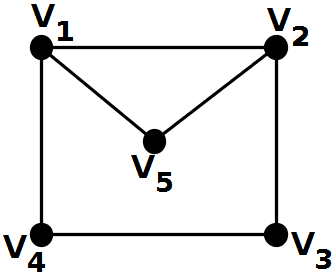
\includegraphics[width=3cm]{./img/envelope.png} & 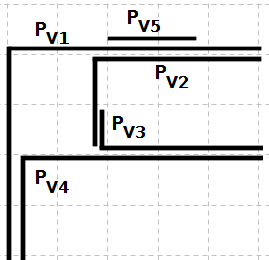
\includegraphics[width=4cm]{./img/envelopeHellyGradeTransparente.png} & 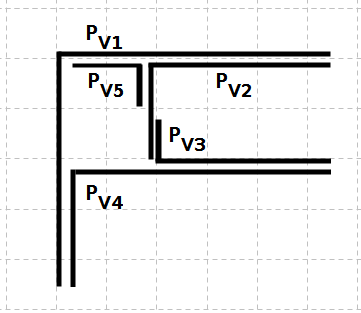
\includegraphics[width=4.6cm]{./img/envelopeNaoHellyGrade.png}
    \\
    \footnotesize \centering (a) Um grafo com  5 vértices & \footnotesize(b) Uma representação $B_1$-EPG que satisfaz a propriedade Helly & \footnotesize (c) Uma representação $B_1$-EPG que não satisfaz a propriedade Helly  \\

  \end{tabular}
\caption{Um grafo com 5 vértices em (a) e algumas representações de dobra simples: uma representação Helly em (b) e outra representação que não satisfaz a propriedade Helly em (c)} \label{fig:envelopeRepresentacoes}
\end{figure}



\subsection{O Estudo de Grafos EPG}

A pesquisa envolvendo grafos de aresta-intersecção de caminhos em grade é tópico relativamente novo na área de Teoria dos Grafos, as primeiras definições formais de problemas e aplicações foram apresentadas por Golumbic em 2009~\cite{golumbic2009}. Desde então diversas questões tem sido investigadas pela comunidade científica. Essas questões frequentemente abordam as representações dos caminhos, restrições quanto ao número de dobras em uma representação, etc.

\begin{table}[h]
\caption{Algumas classes de grafos e limites conhecidos para o \textit{bend-number}}
\label{tab:limitesBenNumber}
\begin{center}
\begin{tabular}{|c|c|c|}
\hline 
Classe de Grafo & b(G) & Referência \\ 
\hline \hline  
Grafos de Intervalo & 0 & \cite{golumbic2009} \\ 
\hline 
Florestas & 1 & \cite{golumbic2009} \\ 
\hline 
Outerplanar & 2 & \cite{daniel2014b} \\ 
% \hline 
% Planar & 5 e dim $(n-1)\times(2n-3)$ & \cite{biedl2010} 2010\\ 
\hline 
Planar & $3 \leq - \leq 4$ & \cite{daniel2014b}\\ 
\hline  
Bipartido Planar & 2 & \cite{biedl2010} \\ 
\hline 
Grafo Linha & 2 & \cite{biedl2010} \\ 
\hline 
dgn(G)~\footnote{Degeneracy - uma orientação acíclica de $G$ que é $k-$regular } $\leq k$ & $2k-1$ & \cite{daniel2014b} \\ 
\hline 
tw(G)~\footnote{Treewidth} $\leq k$ & $2k-2$ & \cite{daniel2014b} \\ 
\hline 
Degree $\leq \Delta$ & $ 	\lceil \frac{\Delta}{2}\rceil\leq - \leq\Delta $ & \cite{daniel2014b} \\ 
\hline 
Arco-circular & 3 & \cite{alcon2016} \\ 
\hline 
\end{tabular} 
\end{center}
\end{table}


\begin{theorem}
Todo grafo planar possui uma representação $B_{5}$-EPG em uma grade $(n-1)\times (2n-3)$.
\end{theorem}

obs 5. Grafos cordais, livres de garra, touro* e diamante possuem uma representação $B_{1}-$EPG, \citep{ries2009}, nesse mesmo paper há uma pequena caracterização de alguns grafos splits.

obs 6. Grafos arco-circulares são $B_{4}-$EPR (retângulos).

obs 7. Em \citep{alcon2016} também há uma caracterização dos grafos $B_{1}-$EPR através de uma família minimal de subgrafos proibidos (que formam uma subclasses de normal arco-circular Helly).

obs 8. Em \citet{cohen2014} é apresentado um algoritmo de reconhecimento de tempo linear para cografos $B_{1}-$EPG e  $B_{0}-$VPG, utilizando sua coárvore.

obs 9. Reconhecimento de $B_{1}-$EPG é NP-completo, \citep{heldt2014}.


Número de dobras em grafos bipartidos completos ($K_{m,n}$)

Em \cite{heldt2014} são apresentados alguns resultados para grafos bipartidos completos. Considerando os limites conhecidos para o número de intervalo (\textit{interval number}) de $K_{m,n}$ e para o número de caminhos (\textit{track number}), sabidamente $i(K_{m,n})= \lceil \frac{mn+1}{m+n} \rceil$ e $t(K_{m,n})= \lceil \frac{mn}{m+n-1} \rceil$, ambas fórmulas fechadas. Em contraste, é difícil obter uma forma fechada para o número de dobras da grade para grafos bipartido completos.


Conjectura de \cite{heldt2014} diz que grafos livres de garra possuem bend number arbitrariamente grande (pag 148, Conjecture 2).

\begin{theorem}
Todo grafo planar possui uma representação 5-EPG em uma grade de tamanho $(n-1)\times(2n-3)$, \cite{biedl2010}.
\end{theorem}

\begin{theorem}
Todo grafo bipartido planar $G=(A\cup B, E)$ possui uma representação 2-EPG em uma grade de tamanho $(|A|+1)\times(|B|+1)$, \cite{biedl2010}.
\end{theorem}

% \begin{proof}
% É conhecido que todo grafo bipartido planar pode ser representado por linhas horizontais e verticais que se tocam, e.e. vértices são atribuídos a segmentos abertos disjuntos de tal forma que $(v,w)$ é uma aresta se e somente se o fecho de segmentos entre $v$ e  $w$ é intersectante. Todavia, pode-se conseguir que estes segmentos estejam em uma grade de ordem $|A|\times |B|$ sem que dois segmentos estejam sobre a mesma linha vertical ou horizontal.

% Dados $s_{h}$ e $s_{v}$ segmentos horizontal e vertical, respectivamente, que se tocam no ponto $(x,y)$. Para pelo menos um deles esse ponto deve ser um ponto final. Se somente $s_{v}$ termina em $(x,y)$, então adicione ao segmento $[x,x+1]\times y$ ao caminho da grade substituindo $s_{v}$.
% Se somente $s_{h}$ termina em $(x,y)$, então adicione ao segmento $x\times [y,y+1]$ ao caminho da grade substituindo $s_{h}$. Se ambos terminarem em $(x,y)$ efetue a adição em ambos.

% Na verdade o que foi feito foi substituir um segmento vertical em ``C'' por um segmento horizontal em ``U''. Exceto para o caso onde ambos os segmentos possuem mesmo ponto final, sempre obtemos dessa forma uma representação 2-EPG com as propriedades desejadas.
% \end{proof}



\begin{theorem}
Todo grafo planar possui uma representação 5-EPG em uma grade de dimensão $(n-1)\times(2n-3)$\cite{biedl2010}.
\end{theorem}




